\section{Programmation système : Multiprocessing}
\textbf{Warning: } Pour cette exercice, il a fallu reconfigurer le noyau linux en activant certaines options. Pour cela, se référer à la slide 72 du support de cours. Cette opération prend un temps considérable.
\subsection{Processus, signaux et communication}
\subsubsection{Exercice 1}
\textbf{Donnée:} Concevez	et	développez	une	petite	application	mettant	en	œuvre	un	des	services	de	communication
proposé	par	Linux	(p.ex.	« socketpair ») entre	un	processus	parent	et	un	processus	enfant.	
Le	processus	enfant	devra	émettre	quelques	messages	sous	forme	de	texte	vers	le	processus	parent,	
lequel	les	affichera	sur	la	console.	Le	message	« exit »	permettra	de	terminer	l’application.
Cette	application	devra	impérativement	capturer	tous	les	signaux	et	les	ignorer.	Seul	un	message	
d’information	sera	affiché	sur	la	console.\\\\
\textbf{Emplacement du code : } \textit{/Multiprocessing/Exercice1-Comm}\\

\textbf{Exécution du code : } \\
Le processus enfant demande à l'utilisateur de tapper quelque chose, qui est ensuite retransmis au parent, qui l'affiche. \\
\begin{lstlisting}
lmi@csel1:~$ cd workspace/csel1/environment/multiproc/exercice1
lmi@csel1:~/workspace/csel1/environment/multiproc/exercice1$ make clean all
\end{lstlisting}

\begin{lstlisting}
# cd /usr/workspace/csel1/environment/multiproc/exercice1/                      
# ./app_a                                                                       
In the main process.                                                            

In the parent process                                                           

In the children process.                                                        

Enter a msg to send to the parent :                                             
Hello                                                                           
Hello will be written to the parent.                                            
Enter a msg to send to the parent :                                             
Received 50 from the children. String is : Hello                                
Bla                                                                             
Bla will be written to the parent.                                              
Enter a msg to send to the parent :                                             
Received 50 from the children. String is : Bla                                  
Received signal is : Interrupt                                                 
Received signal is : Interrupt                                                  
Bla will be written to the parent.                                              
Enter a msg to send to the parent :                                             
Received 50 from the children. String is : Bla                                  
Received signal is : Stopped                                                    
Received signal is : Stopped                                                    
Bla will be written to the parent.                                              
Enter a msg to send to the parent :                                             
Received 50 from the children. String is : Bla                                  
exit                                                                          
exit will be written to the parent.                                             
Received 50 from the children. String is : exit 
#
\end{lstlisting}
Ce second output montre que le SIGINT est géré pour afficher un message en écrivant \textit{Received signal is :} suivi du type de signal. Dans le cas suivant, c'est un ctrl-c qui a été envoyé. 
\begin{lstlisting}
Enter a msg to send to the parent : Received 50 from the children. String is : 
^CReceived signal is : Interrupt
Received signal is : Interrupt
will be written to the parent.
Enter a msg to send to the parent : Received 50 from the children. String is : 
\end{lstlisting}

\subsection{CGroups}
\subsubsection{Exercice 2}
\textbf{Donnée:} Concevez	une	petite	application	permettant	de	valider	la	capacité	des	groupes	de	contrôle	de	limiter	
l’utilisation	de	la mémoire.	\\\\

\textbf{Emplacement du code : } \textit{/Multiprocessing/Exercice2-cgroups}\\

\textbf{Réponse aux questions :}\\

\textbf{a.Quel effet a la commande <<echo \$\$ > ...>> sur les cgroups?}\\
Par cette commande, on demande aux cgroups de surveiller la tache représentée par le terminal de l'ordroid. Comme le programme que nous lançons depuis la ligne de commande devient le fils du terminal dans lequel il est lancé, on surveille aussi le fils car il est automatiquement affecté à la hiérarchie du parent. \\\\

\textbf{b.Quel est le comportement du sous-système <<memory>> lorsque le quota de mémoire est épuisé? Pourrait-on le modifier? Si oui, comment?}\\
Le comportement par défaut est de tuer le processus dépassant les limites. Mais il est possible de modifier ce comportement en mettant un \textbf{1} dans <<memory.oom\_control>>. Si la modification a été apportée, le processus qui viendrait à dépasser les limites de mémoire se verrait mis en pause.\\

L'output en dessous montre qu'une fois le programme \textit{app\_a} lancé, après vingt allocations, il est tué à cause de son excès de consommation mémoire. 
\begin{lstlisting}
# ./app_a 
Ten more megas allocated

Ten more megas allocated

Killed
\end{lstlisting}


\textbf{c.Est-il possible de surveiller/vérifier l'état actuel de la mémoire? Si oui, comment?}\\
Plusieurs commandes peuvent être utilisées pour visualiser l'état de la mémoire :
\begin{itemize}
	\item \textit{free -m}
	\item \textit{cat /proc/meminfo}
\end{itemize}
La première produit ce genre d'output:
\begin{lstlisting}
# free -m
total        used        free      shared  buff/cache   available
Mem:           1990         156        1808           0          24        1813
Swap:             0           0           0
\end{lstlisting}
Tandis que la seconde produit ça :
\begin{lstlisting}
# cat /proc/meminfo 
MemTotal:        2038540 kB
MemFree:         1852220 kB
Buffers:               0 kB
Cached:             5272 kB
SwapCached:            0 kB
Active:             3308 kB
Inactive:           2952 kB
Active(anon):       1012 kB
Inactive(anon):       88 kB
Active(file):       2296 kB
Inactive(file):     2864 kB
Unevictable:           0 kB
Mlocked:               0 kB
HighTotal:       1296384 kB
HighFree:        1147292 kB
LowTotal:         742156 kB
LowFree:          704928 kB
SwapTotal:             0 kB
SwapFree:              0 kB
Dirty:                 0 kB
Writeback:             0 kB
AnonPages:          1000 kB
Mapped:             2084 kB
Shmem:               112 kB
Slab:              20200 kB
SReclaimable:       9264 kB
SUnreclaim:        10936 kB
KernelStack:         840 kB
PageTables:          124 kB
NFS_Unstable:          0 kB
Bounce:                0 kB
WritebackTmp:          0 kB
CommitLimit:     1019268 kB
Committed_AS:       5752 kB
VmallocTotal:     245760 kB
VmallocUsed:       16520 kB
VmallocChunk:     103580 kB
\end{lstlisting}
Si on veut monitorer la consommation de notre application, on peut aussi utiliser Valgrind et l'outil \textit{massif} avec la commande suivante : 
\begin{lstlisting}
valgrind --tool=massif ./app_a
\end{lstlisting}
Le programme s'execute normalement et l'outil de visualisation produit un fichier contenant tout le logging de la mémoire utilisée par l'application. On peut la voir avec la commande :
\begin{lstlisting}
ms_print massif.out.<app_a pid>
\end{lstlisting}
Ce qui produit dans notre cas :
\begin{lstlisting}
--------------------------------------------------------------------------------
Command:            ./app_a
Massif arguments:   (none)
ms_print arguments: massif.out.1695
--------------------------------------------------------------------------------


MB
47.68^                                                                      :#
|                                                                   ::@:#
|                                                               ::::: @:#
|                                                            ::::: :: @:#
|                                                        :::::: :: :: @:#
|                                                     :@@:: ::: :: :: @:#
|                                                 :::::@ :: ::: :: :: @:#
|                                              ::::: ::@ :: ::: :: :: @:#
|                                          :::::: :: ::@ :: ::: :: :: @:#
|                                       :@@::: :: :: ::@ :: ::: :: :: @:#
|                                  ::::::@ ::: :: :: ::@ :: ::: :: :: @:#
|                                ::: :: :@ ::: :: :: ::@ :: ::: :: :: @:#
|                           :::::::: :: :@ ::: :: :: ::@ :: ::: :: :: @:#
|                        ::@: :: ::: :: :@ ::: :: :: ::@ :: ::: :: :: @:#
|                    ::::: @: :: ::: :: :@ ::: :: :: ::@ :: ::: :: :: @:#
|                 :::: ::: @: :: ::: :: :@ ::: :: :: ::@ :: ::: :: :: @:#
|             ::::: :: ::: @: :: ::: :: :@ ::: :: :: ::@ :: ::: :: :: @:#
|          ::@:: :: :: ::: @: :: ::: :: :@ ::: :: :: ::@ :: ::: :: :: @:#
|       :::: @:: :: :: ::: @: :: ::: :: :@ ::: :: :: ::@ :: ::: :: :: @:#
|     ::: :: @:: :: :: ::: @: :: ::: :: :@ ::: :: :: ::@ :: ::: :: :: @:#
0 +----------------------------------------------------------------------->Mi
0                                                                   13.57

...
\end{lstlisting}
Pour nous rassurer, avec la commande et l'output suivant, on constate quand même que la mémoire a bien été libérée:
\begin{lstlisting}
# valgrind ./app_a 
==1701== Memcheck, a memory error detector
==1701== Copyright (C) 2002-2013, and GNU GPL'd, by Julian Seward et al.
==1701== Using Valgrind-3.10.0 and LibVEX; rerun with -h for copyright info
==1701== Command: ./app_a
==1701== 
Ten more megas allocated

Ten more megas allocated

Ten more megas allocated

Ten more megas allocated

Press enter to continue...


Ten more megas freed

Ten more megas freed

Ten more megas freed

Ten more megas freed

Ten more megas freed

==1701== 
==1701== HEAP SUMMARY:
==1701==     in use at exit: 0 bytes in 0 blocks
==1701==   total heap usage: 50 allocs, 50 frees, 50,000,000 bytes allocated
==1701== 
==1701== All heap blocks were freed -- no leaks are possible
==1701== 
==1701== For counts of detected and suppressed errors, rerun with: -v
==1701== ERROR SUMMARY: 0 errors from 0 contexts (suppressed: 0 from 0)
\end{lstlisting}
Pour les derniers outputs, la limite d'allocation mémoire a été élevée à 100MB. Aucune solution n'a été trouvée autrement pour monitorer la mémoire du processus durant son exécution avec le contrôle de la mémoire. Valgrind est autant tué que l'application, sinon.

\subsubsection{Exercice 3}
\textbf{Donnée:} Afin	valider	la	capacité	des	groupes	de	contrôle	de	limiter	l’utilisation	des	CPU,	concevez	une	petite	application	composée	au	minimum	de	2	processus	utilisant	le	100\%	des	ressources	du	processeur.	\\\\

\textbf{Emplacement du code : } \textit{/Multiprocessing/Exercice3-CPU}\\

\textbf{Monter les cgroup : } \\
\begin{lstlisting}
# mount -t tmpfs none /sys/fs/cgroup                                            
# mkdir /sys/fs/cgroup/memory                                                   
# mount -t cgroup -o memory memory /sys/fs/cgroup/memory                        
# mkdir /sys/fs/cgroup/memory/mem         
# mkdir /sys/fs/cgroup/cpuset                                                   
# mount -t cgroup -o cpu,cpuset cpuset /sys/fs/cgroup/cpuset                    
# mkdir /sys/fs/cgroup/cpuset/high         
# mkdir /sys/fs/cgroup/cpuset/low  
# echo 4 > /sys/fs/cgroup/cpuset/high/cpuset.cpus                               
# echo 0 > /sys/fs/cgroup/cpuset/high/cpuset.mems                               
# echo 3 > /sys/fs/cgroup/cpuset/low/cpuset.cpus                                
# echo 0 > /sys/fs/cgroup/cpuset/low/cpuset.mems                                 
\end{lstlisting}

\textbf{Réponse aux questions :}\\\\
\textbf{a. Les	4	dernières	lignes	sont	obligatoires	pour que	les	prochaines	commandes	fonctionnent	
	correctement. Pouvez-vous	en	donner	la	raison ?}\\\\
Les deux commandes écrivant dans le cpuset.cpus assignent un numéro de cœur pour le cpuset. Les autres écrivant dans le cpuset.mems limite l'espace mémoire et le crée. Cela crée l'architecture du CGroups. Pour l'avoir testé, si on n'affecte pas un cpuset.mems, l'application n'a pas de place en mémoire.
\begin{lstlisting}
# echo $$ > /sys/fs/cgroup/cpuset/low/tasks
sh: write error: No space left on device
\end{lstlisting}

\textbf{b. Ouvrez	deux	shells	distincte	et	placez en	une	dans	le	cgroup	high	et	l’autre	dans	le	cgroup	low.\\	
	Lancez	ensuite	votre	application	dans	chacune	des	shells.\\
	Quel	devrait	être	le	bon	comportement ?	Pouvez-vous	le	vérifier ?}\\\\
Installation de l'application avec la connexion sérielle: \\
Oui, on peut le vérifier, les commandes sont visibles un peu plus loin. Le comportement attendu est une utilisation à 100\% des cœurs 3 et 4 (attribués lors de la création du CGroup) du processeur avec 50\% pour le parent et 50\% pour le parent. Pour l'instant, on n'a pas assigné de limitation dans l'utilisation du temps CPU.\\
\begin{lstlisting}
lmi@csel1:~$ sudo minicom
...
# echo $$ > /sys/fs/cgroup/cpuset/high/tasks                                    
# ./app_a                                                                       
In the main process.                                                            

In the parent process                                                           

In the children process.  
\end{lstlisting}
Installation de l'application avec la connexion ssh: \\
\begin{lstlisting}
lmi@csel1:~$ ssh root@192.168.0.11
# echo $$ > /sys/fs/cgroup/cpuset/low/tasks
# cd /usr/workspace/csel1/environment/multiproc/exercice3/
# echo $$ > /sys/fs/cgroup/cpuset/low/tasks    
# ./app_a 
In the main process.

In the parent process

In the children process.

\end{lstlisting}

L'utilisation du CPU peut être affichée avec la commande top en lançant l'application en arrière plan:\\
\begin{lstlisting}
# ./app_a &                                                                     
# In the main process.                                                          

In the parent process                                                           

In the children process.  

# top
\end{lstlisting}

\begin{figure}[H]
	\begin{center}
		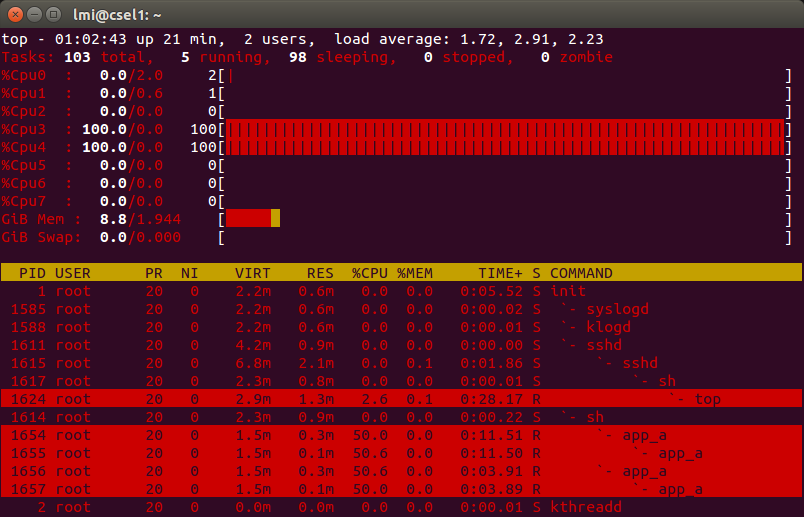
\includegraphics[width=16cm]{img/multiprocessCGroup.png}
		\caption{Utilisation du processeur}
		\label{multiprocess1}
	\end{center}
\end{figure}
\textbf{c. Sachant	que	l’attribut	cpus.shares permet	de	répartir	le	temps	CPU	entre	différents	
	cgroups,	comment devrait-on	procéder	pour	lancer deux	tâches	distinctes	sur	le	cœur	6	de	
	notre	processeur	et	attribuer	75\%	du	temps	CPU	à	la	première	tâche	et	25\%	à	la	deuxième ?}\\\\
Voici les commandes utilisées pour la configuration demandée. Par défaut, l'attribut cpu.shares contient 1024, qui représente 50\% du temps CPU. Pour plus de lisibilité, l'application a été compilée une fois sous le nom app\_a et une fois sous le nom app\_b.\\\\
Dans la connection ssh:
\begin{lstlisting}
# top
\end{lstlisting}
Dans la connection série:
\begin{lstlisting}
# echo 512 > /sys/fs/cgroup/cpuset/low/cpu.shares 
# echo 1536 > /sys/fs/cgroup/cpuset/high/cpu.shares  
# echo $$ > /sys/fs/cgroup/cpuset/low/tasks                                     
# ./app_b &                                                                     
# In the main process.                                                          

In the parent process                                                           

In the children process.                                                        

# echo $$ > /sys/fs/cgroup/cpuset/high/tasks                                    
# ./app_a &                                                                     
# In the main process.                                                          

In the parent process                                                           

In the children process.                                                        

# 
\end{lstlisting}
Voici le résultat obtenu, l'app\_a prend 75\% du temps CPU (37.7\% parent, 37.7\% enfant) et l'app\_b 25\%.
\begin{figure}[H]
	\begin{center}
		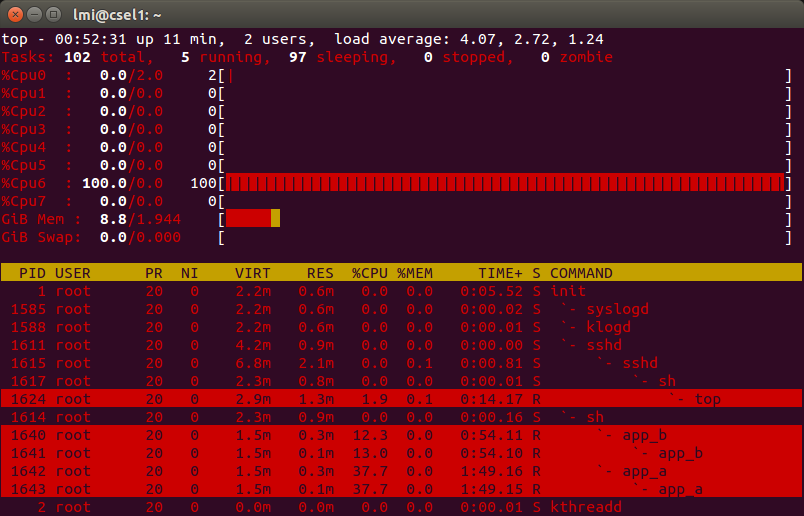
\includegraphics[width=16cm]{img/multiprocessCGroup2.png}
		\caption{Répartition du temps processeur}
		\label{multiprocess2}
	\end{center}
\end{figure}
